

\tikzset{every picture/.style={line width=0.75pt}} %set default line width to 0.75pt        

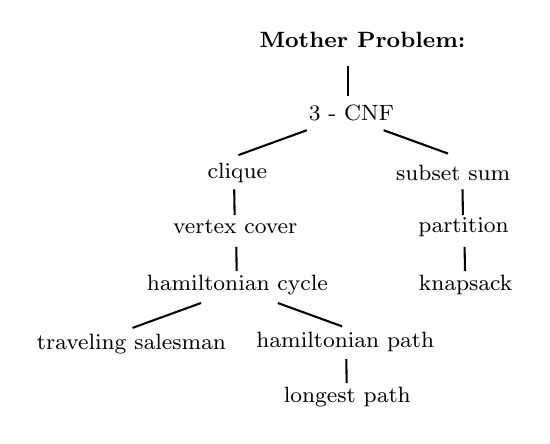
\begin{tikzpicture}[x=0.75pt,y=0.75pt,yscale=-0.75,xscale=1]
%uncomment if require: \path (0,278); %set diagram left start at 0, and has height of 278

%Straight Lines [id:da5140465997472392] 
\draw    (311.3,40.2) -- (311.3,59.2) ;
%Straight Lines [id:da8208289180892083] 
\draw    (291.3,81.2) -- (258.3,97.2) ;
%Straight Lines [id:da968472968777252] 
\draw    (359.3,96.2) -- (328.3,81.2) ;
%Straight Lines [id:da4226687837322394] 
\draw    (366.5,135.71) -- (366.3,119.2) ;
%Straight Lines [id:da8434647434252256] 
\draw    (367.5,171.71) -- (367.3,156.2) ;
%Straight Lines [id:da3568330391803052] 
\draw    (256.5,135.71) -- (256.3,119.2) ;
%Straight Lines [id:da8259647253172495] 
\draw    (257.5,171.71) -- (257.3,156.2) ;
%Straight Lines [id:da44899188855816097] 
\draw    (240.3,192.2) -- (207.3,208.2) ;
%Straight Lines [id:da5229375564759453] 
\draw    (308.3,207.2) -- (277.3,192.2) ;
%Straight Lines [id:da3723435334118188] 
\draw    (310.5,243.71) -- (310.3,228.2) ;

% Text Node
\draw (267,16) node [anchor=north west][inner sep=0.75pt]   [align=left] {{\footnotesize \textbf{Mother Problem:}}};
% Text Node
\draw (312.8,70.4) node  [font=\footnotesize] [align=left] {{\footnotesize 3 - CNF}};
% Text Node
\draw (257.8,108.4) node  [font=\footnotesize] [align=left] {{\footnotesize clique}};
% Text Node
\draw (361.8,108.4) node  [font=\footnotesize] [align=left] {{\footnotesize subset sum}};
% Text Node
\draw (366.8,143.4) node  [font=\footnotesize] [align=left] {{\footnotesize partition}};
% Text Node
\draw (367.8,180.4) node  [font=\footnotesize] [align=left] {{\footnotesize knapsack}};
% Text Node
\draw (256.8,143.4) node  [font=\footnotesize] [align=left] {{\footnotesize vertex cover}};
% Text Node
\draw (257.8,180.4) node  [font=\footnotesize] [align=left] {{\footnotesize hamiltonian cycle}};
% Text Node
\draw (309.8,217.4) node  [font=\footnotesize] [align=left] {{\footnotesize hamiltonian path}};
% Text Node
\draw (206.8,218.4) node  [font=\footnotesize] [align=left] {{\footnotesize traveling salesman}};
% Text Node
\draw (310.8,252.4) node  [font=\footnotesize] [align=left] {{\footnotesize longest path}};


\end{tikzpicture}